\documentclass[a4paper]{article}
\usepackage{graphicx}

\begin{document}
\title{The TraGit DuckTale}
\author{F.dev}
\maketitle

\section*{Kapitel 1}
Det var en gång en badanka som heter Anki och en programmerare som heter % TODO lägg till ditt namn
Klockan var efter midnatt och programmeraren brottades med en synnerligen svåridentifierad bug.

\begin{center}
	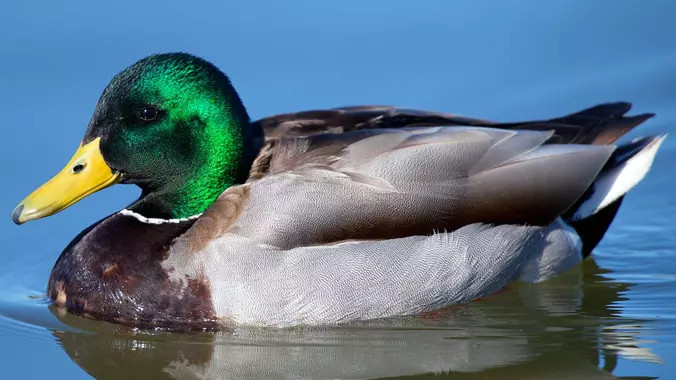
\includegraphics[scale=0.3]{duck_that_is_not_anki.jpeg}
\end{center}

% TODO beskriv programmet!

\section*{Kapitel 3}
Bland allt svett och alla tårar som samlats på golvet fick Anki flyt. Då hände det! Programmeraren kom till slutet av filen och såg där:

\texttt{main}

Inga parenteser. Programmet började inte ens vid körning. Totalt chanslös att utföra ens den enklaste operationen. Med en djup suck av lättnad lade hen till parenteserna, och programmet kördes perfekt.

\end{document}
